\documentclass[a2paper]{article}

\usepackage{siunitx}
\usepackage{tikz}
\usepackage{amsmath}
\usepackage{geometry}
% \usepackage{showframe}

\geometry{a2paper,margin=0.5in}
\pagestyle{empty}

\begin{document}
\thispagestyle{empty}

\begin{figure}[h!]
\begin{tikzpicture}
\node[anchor=south west,inner sep=0] at (0.2,-5.0) 
{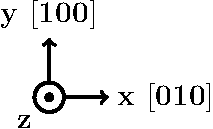
\includegraphics[width=0.30\textwidth]{arrows1}};
\node[anchor=south west,inner sep=0] at (0.2,0.0)  
{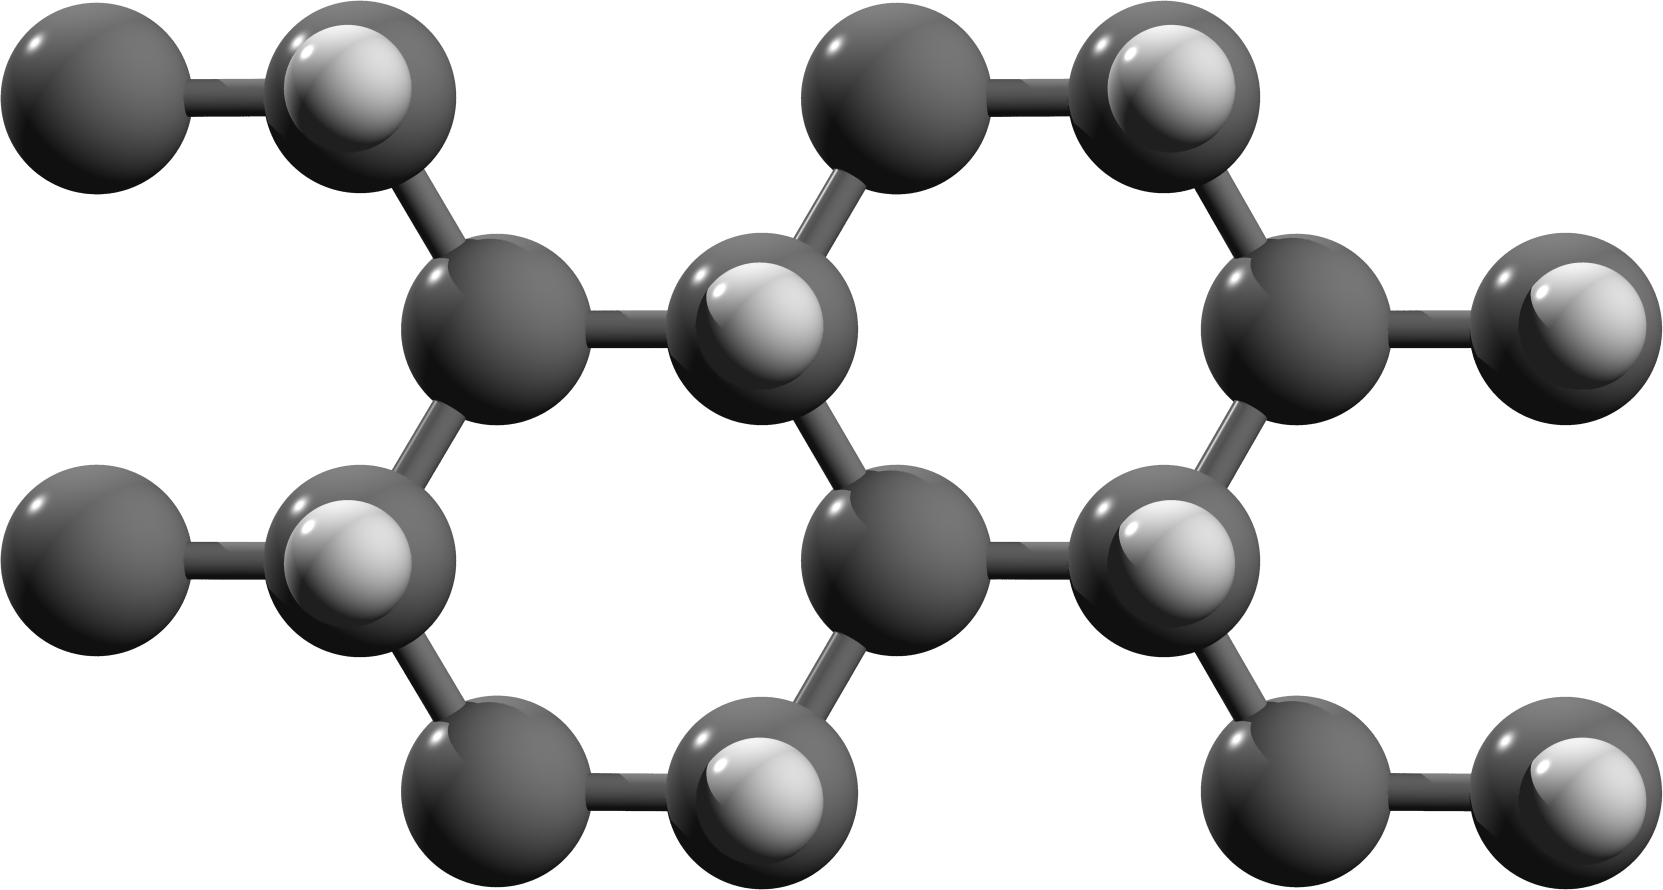
\includegraphics[width=\textwidth]{up1}};
\draw [line width=2.00mm, red ] (-0.30,05.00) -- (-0.30,10.60) node [right] {};
\draw [line width=2.00mm, red ] (-0.30,10.50) -- (10.50,10.50) node [right] {};
\draw [line width=2.00mm, red ] (10.45,10.55) -- (13.75,05.00) node [right] {};
\draw [line width=2.00mm, red ] (13.67,05.00) -- (21.00,05.00) node [right] {};
\draw [line width=2.00mm, red ] (21.05,05.10) -- (21.05,-0.60) node [right] {};
\draw [line width=2.00mm, red ] (10.30,-0.50) -- (21.00,-0.50) node [right] {};
\draw [line width=2.00mm, red ] (07.01,05.15) -- (10.38,-0.55) node [right] {};
\draw [line width=2.00mm, red ] (-0.30,05.10) -- (07.08,05.10) node [right] {};
\node[anchor=south west,inner sep=0] at (0.2,-20.0) 
{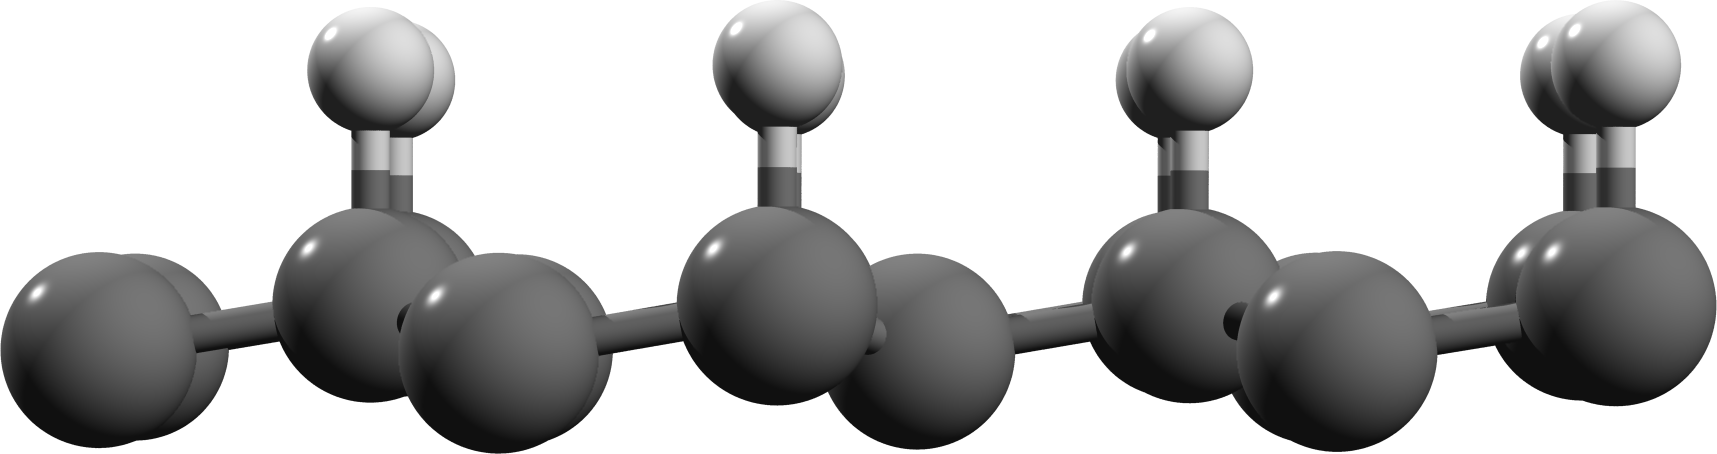
\includegraphics[width=\textwidth]{up2}};
\node[anchor=south west,inner sep=0] at (0.2,-34.0) 
{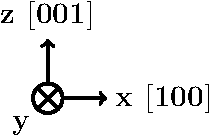
\includegraphics[width=0.30\textwidth]{arrows2}};
\draw [line width=2.00mm, red ](-0.30,-20.70) -- (-0.30,-08.85) node [right]{};
\draw [line width=2.00mm, red ](-0.30,-08.95) -- (21.00,-08.95) node [right]{};
\draw [line width=2.00mm, red ](21.00,-20.70) -- (21.00,-08.85) node [right]{};
\draw [line width=2.00mm, red ](-0.30,-20.60) -- (21.00,-20.60) node [right]{};
\end{tikzpicture}
\end{figure}

\end{document}
